%% Verze pro jednostranný tisk:
% Okraje: levý 40mm, pravý 25mm, horní a dolní 25mm
% (ale pozor, LaTeX si sám přidává 1in)
\documentclass[12pt,a4paper]{article}

% \openright zařídí, aby následující text začínal na pravé straně knihy
\let\openright=\clearpage

%% Pokud tiskneme oboustranně:
% \documentclass[12pt,a4paper,twoside,openright]{report}
% \setlength\textwidth{145mm}
% \setlength\textheight{247mm}
% \setlength\oddsidemargin{14.2mm}
% \setlength\evensidemargin{0mm}
% \setlength\topmargin{0mm}
% \setlength\headsep{0mm}
% \setlength\headheight{0mm}
% \let\openright=\cleardoublepage

%% Vytváříme PDF/A-2u
\usepackage[a-2u]{pdfx}

%% Přepneme na českou sazbu a fonty Latin Modern
\usepackage[slovak]{babel}
\usepackage{lmodern}
\usepackage[IL2]{fontenc}%T1
\usepackage{textcomp}
\usepackage{hyperref}

\usepackage{float}
\usepackage{subfigure}

%% Použité kódování znaků: obvykle latin2, cp1250 nebo utf8:
\usepackage[utf8]{inputenc}

%%% Další užitečné balíčky (jsou součástí běžných distribucí LaTeXu)
\usepackage{amsmath}        % rozšíření pro sazbu matematiky
\usepackage{amsfonts}       % matematické fonty
\usepackage{amsthm}         % sazba vět, definic apod.

%bolo treba vypnut kvoli rozdelovaniu
%\usepackage{bbding}         % balíček s nejrůznějšími symboly
% (čtverečky, hvězdičky, tužtičky, nůžtičky, ...)
\usepackage{bm}             % tučné symboly (příkaz \bm)
\usepackage{graphicx}       % vkládání obrázků
\usepackage{fancyvrb}       % vylepšené prostředí pro strojové písmo
\usepackage{indentfirst}    % zavede odsazení 1. odstavce kapitoly
%\usepackage{natbib}         % zajištuje možnost odkazovat na literaturu
% stylem AUTOR (ROK), resp. AUTOR [ČÍSLO]
\usepackage[nottoc]{tocbibind} % zajistí přidání seznamu literatury,
% obrázků a tabulek do obsahu
\usepackage{icomma}         % inteligetní čárka v maltematickém módu
\usepackage{dcolumn}        % lepší zarovnání sloupců v tabulkách
\usepackage{booktabs}       % lepší vodorovné linky v tabulkách
\usepackage{paralist}       % lepší enumerate a itemize
\usepackage[usenames]{xcolor}  % barevná sazba

\usepackage{url}

\usepackage{pdfpages}
%opening
\title{}
\author{}

\begin{document}
	\pagestyle{empty}
\section{Splay}

\subsection{Štandardná implementácia v podmnožinovom teste}

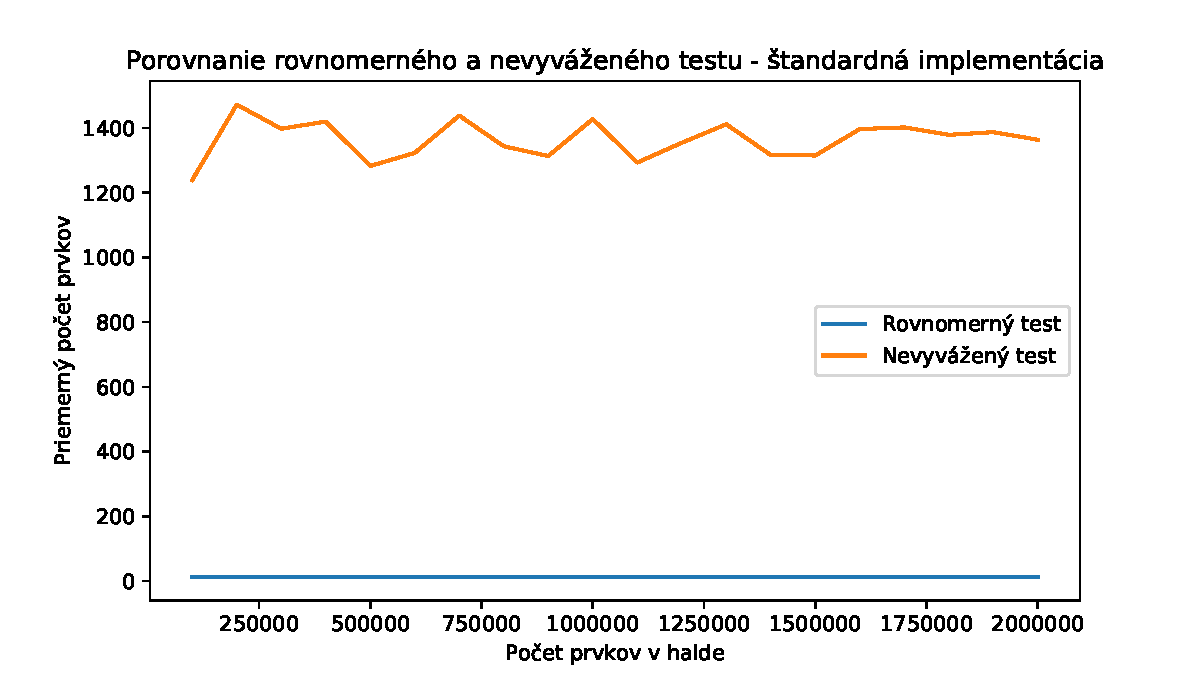
\includegraphics[width=\linewidth]{install/1.pdf}

Z grafu vidíme, správanie Splay stromu, keď v ňom vyhľadávame stále tie isté prvky dokola. Vidíme, že zložitosť vyhľadávania nezáleží na celkovom počte prvkov v strome $n$, ale iba na veľkosti vyhľadávanej množiny. Samozrejme, ak je v strome menej prvkov ako je veľkosť množiny $T$, čas vyhľadania je menší. To vysvetľuje krivku pre $T$ = 1 000 000. Všimnime si, že aj krivka pre $T$ = 100 000 je na začiatku zakrivená, a približne od n ~= 100 000 už zostáva konštantná. Pre $n$ menšie ako $T$ čas stúpa logaritmicky, pre $n$ > $T$ zostáva konštantný. To je z toho dôvodu, že všetky vyhľadávané prvky sa operáciou splay posunú blízko koreňa.

Ten istý graf v logaritmickej mierke:

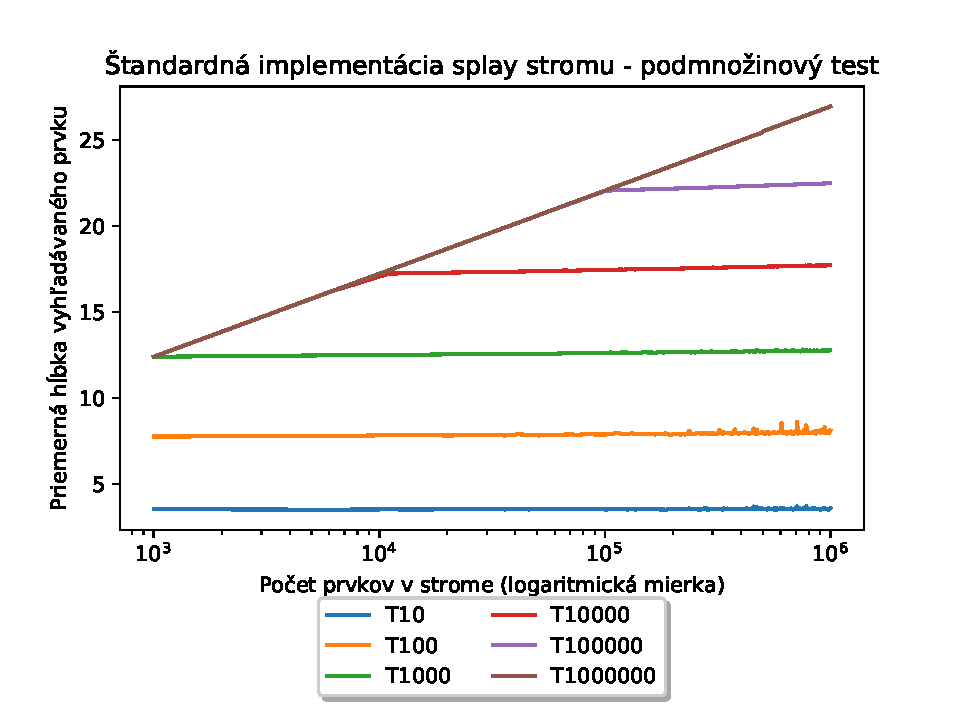
\includegraphics[width=\linewidth]{install/1log.pdf}

\subsection{Naivná implementácia v podmnožinovom teste}

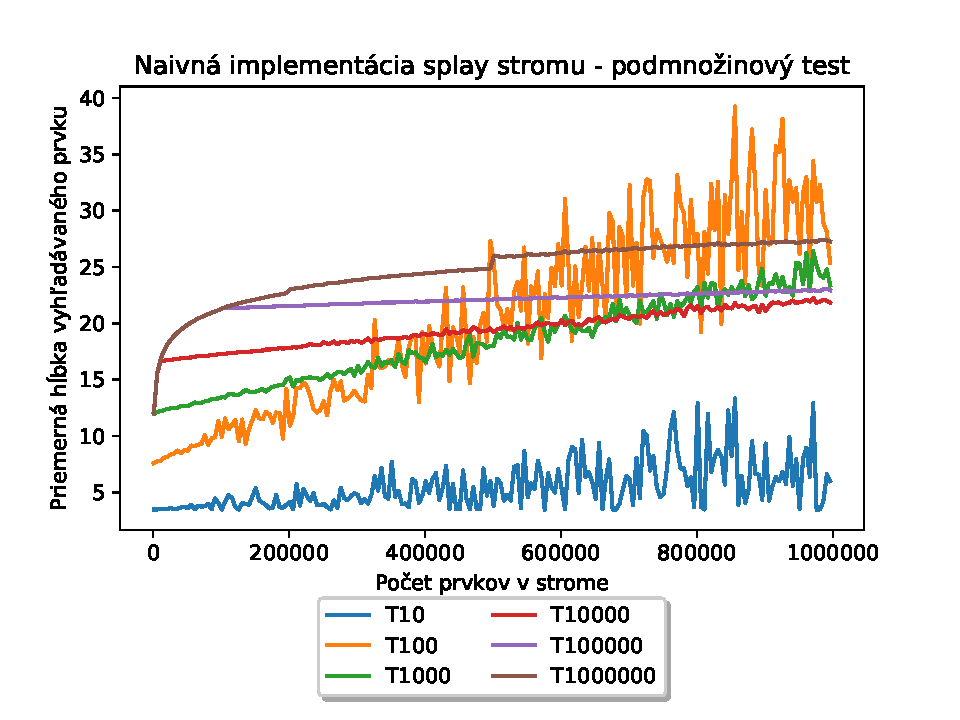
\includegraphics[width=\linewidth]{install/2.pdf}

Na tých istých vstupných dátach ako v predchodzom prípade sme spustili aj naivnú implementáciu splay stromu. Priemerná hĺbka vyhľadávaného prvku je menej predvídateľná. Okrem toho môžeme odhadnúť, že zložitosť operácie find závisí na celkovom počte prvkov v strome. Je to najviditeľnejšie pre $T$ = 100. Naivný splay pravdepodobne nedokáže udržať vyhľadávané prvky blízko koreňa. 

\subsection{Porovnanie naivnej a štandardnej implementácie v podmnožinovom teste}

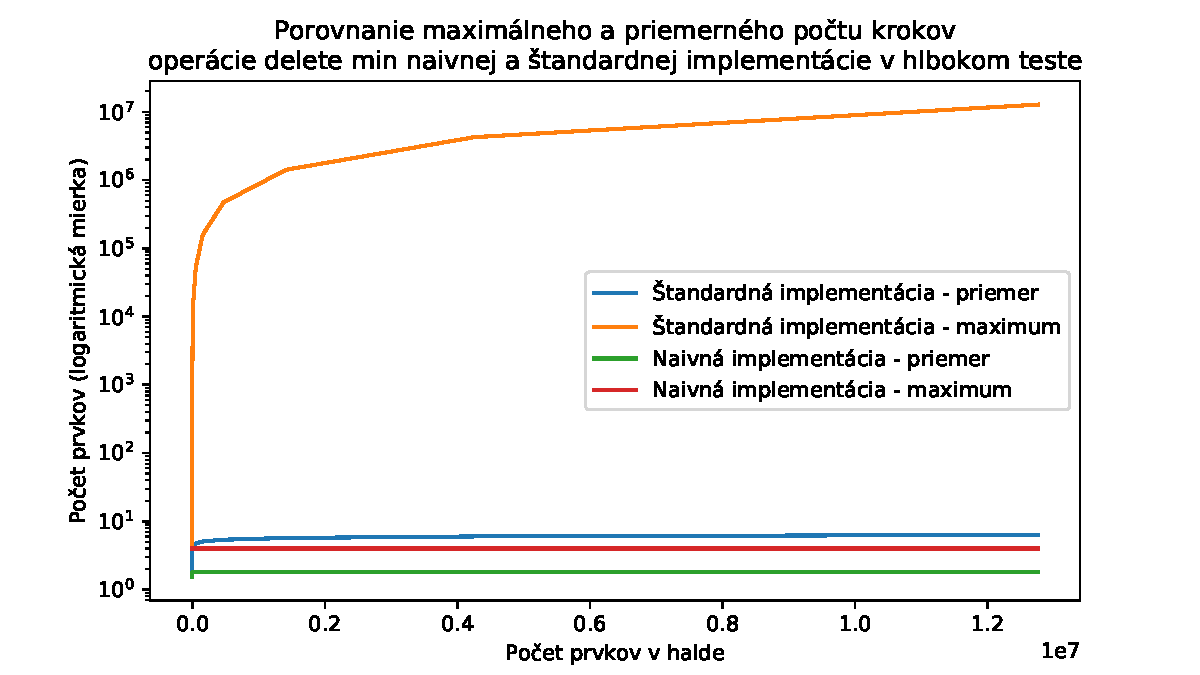
\includegraphics[width=\linewidth]{install/3.pdf}

Porovnanie naivnej a štandardnej implementácie dopadlo lepšie pre štandard. Pre malý počet prvkov v strome pozorujeme mierne lepšiu naivnú implementáciu pri $T$ = 10 000 a $T$ = 1 000 000.

\subsection{Porovnanie štandardnej implementácie a staticky optimálneho stromu v uniformnom teste}
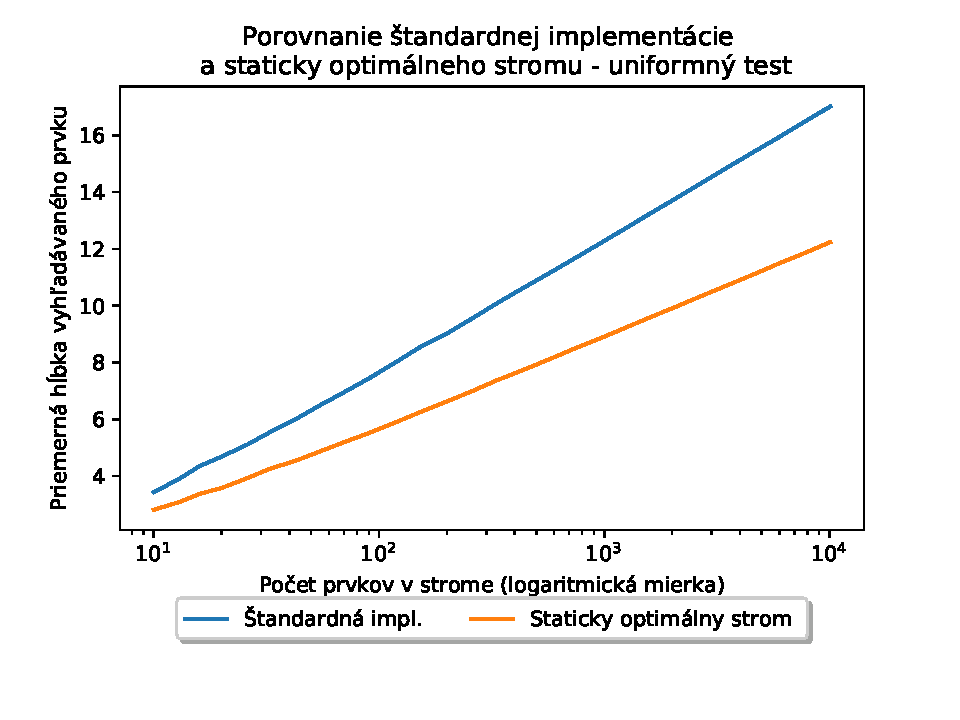
\includegraphics[width=\linewidth]{install/4.pdf}

Z grafu pozorujeme, že s počtom prvkov v strome rastie hĺbka logaritmicky pri oboch stromoch, pri Splay strome rastie rýchlejšie. Odhadol som multiplikatívne konštanty jednoducho tým, že v každom nameranom bode som výslednú hĺbku podelil logaritmom počtu prvkov v strome a následne spriemeroval:
\begin{itemize}
	\item Konštanta pri štandardnej implementácii: 1.18
	\item Konštanta pri staticky optimálnom strome: 1.03
\end{itemize}

%res_s_uniform 1.1821894250138842
%res_o_uniform 1.0283938970638817
%res_s_nonuniform 0.6232486259486356
%res_o_nonuniform 0.5418725190056798

\subsection{Porovnanie štandardnej implementácie a staticky optimálneho stromu v neuniformnom teste}
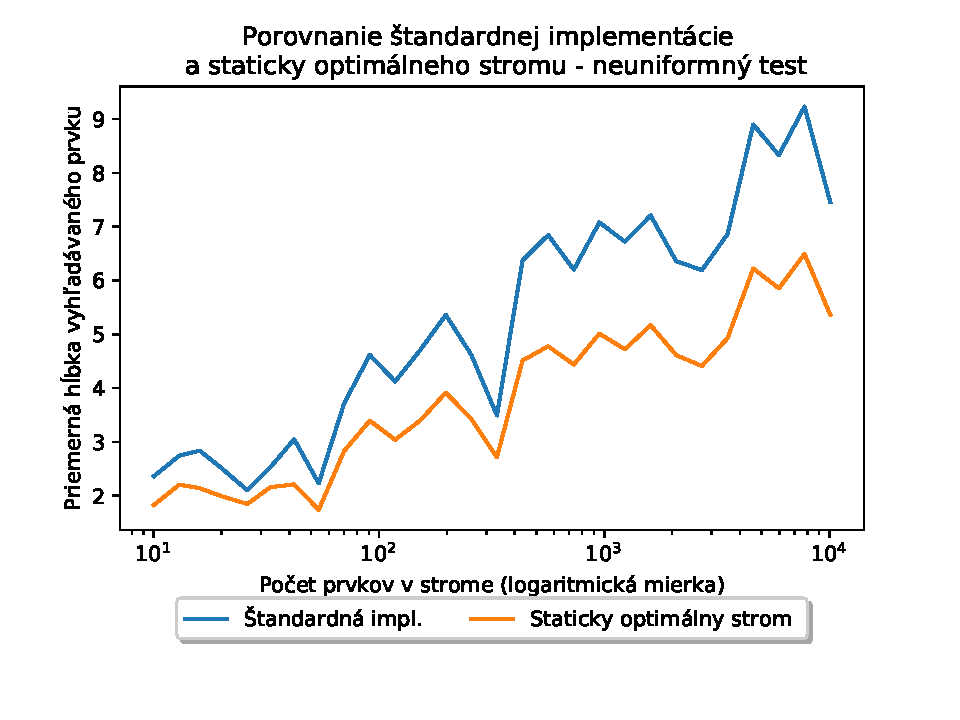
\includegraphics[width=\linewidth]{install/5.pdf}

Pri neuniformnom teste je ťažké odhadnúť akýkoľvek trend, pretože priemerná hĺbka vyhľadávaného prvku príliš závisí na rozdelení vstupných dát a to zahmlieva závislosť na počte prvkov v strome.

Experiment potvrdzuje vetu z prednášky, že splay strom urobí asymptoticky rovnako veľa operácii ako staticky optimálny strom. Optimálny strom má síce vždy menší priemer, ale vždy keď sme namerali menšiu hodnotu pre staticky optimálny strom, namerali sme umerne menšiu hodnotu aj pri splay strome.

\subsection{Porovnanie štandardnej a naivnej implementácie stromu v sekvenčnom teste teste}

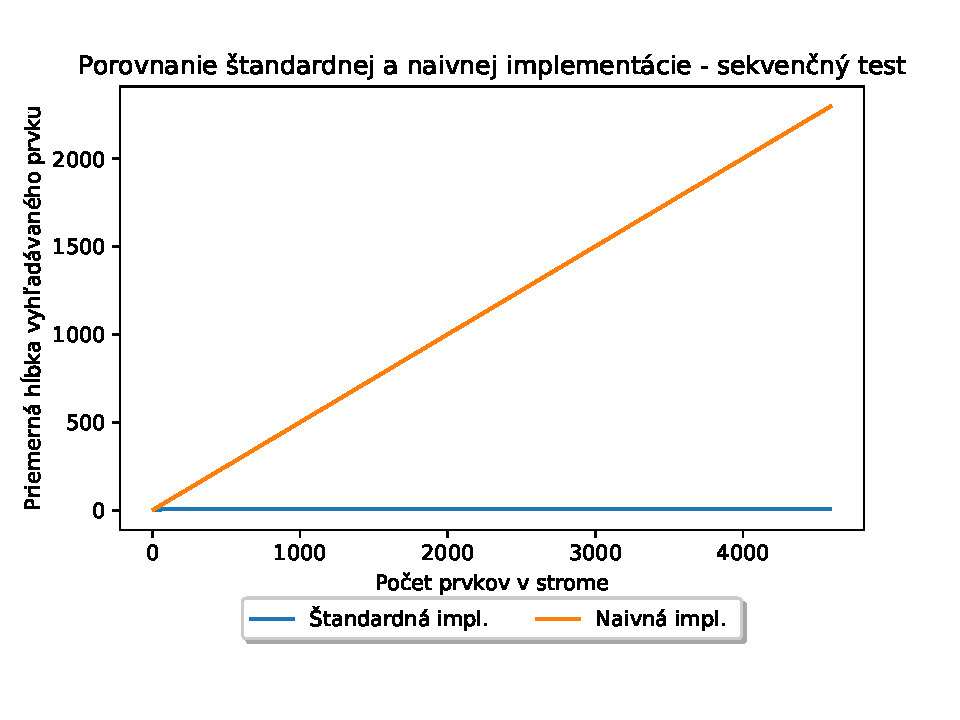
\includegraphics[width=\linewidth]{install/6.pdf}

Namerané hodnoty štandardnej implementácie korešpondujú s vetou z prednášky, že ak postupnosť vyhľadávaní obsahuje rastúce prvky tak celkový čas na vyhľadanie je konštantný.

Priemerná hĺbka vyhľadania naivnej implementácie rastie lineárne.

\subsection{Porovnanie štandardnej implementácie a staticky optimálneho stromu v sekvenčnom teste}

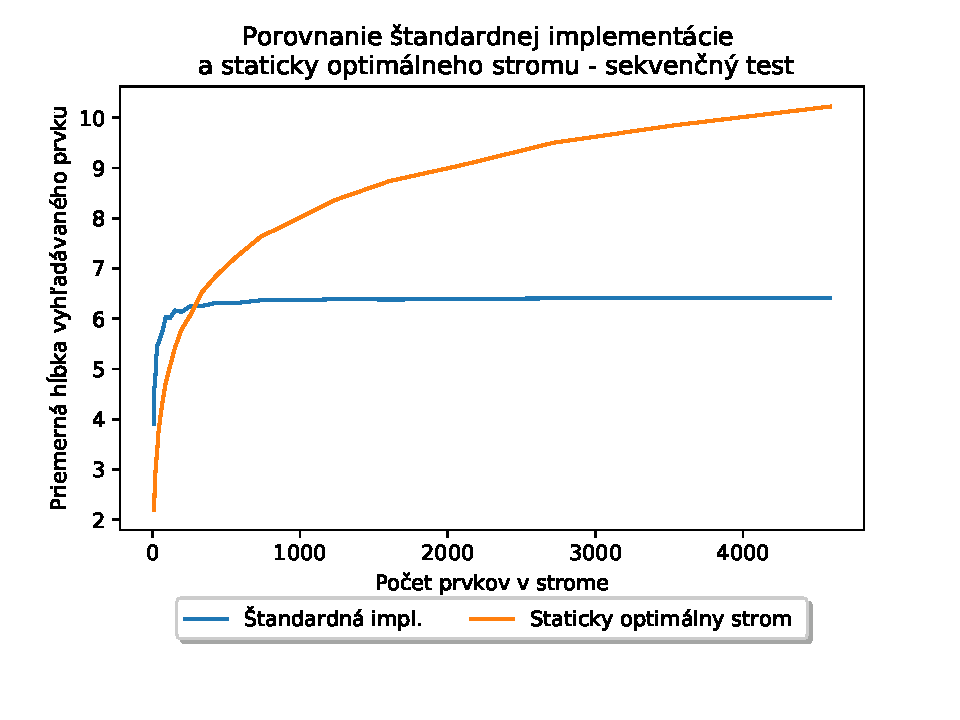
\includegraphics[width=\linewidth]{install/7.pdf}

Splay strom má v tomto porovnaní ``výhodu'' v tom, že sa môže dynamicky upravovať počas vyhľadávania. Priemerná hĺbka vyhľadania v staticky optimálnom strome rastie aj pri sekvenčnom teste logaritmicky. 

\end{document}